\documentclass{article}
\usepackage[margin = 0.15in,landscape]{geometry}
%\usepackage{wasysym}
\usepackage{multicol}
\usepackage{array}
\usepackage{amsmath}
\usepackage{amssymb}
\usepackage{lmodern}
\usepackage{graphicx}
\usepackage{enumitem}
\usepackage{stix}
\usepackage{mathrsfs}
\setlength\parindent{0pt}
\renewcommand{\baselinestretch}{0.75}

\begin{document}
\begin{multicols*}{3}
    Marissa Palamara\par 
    ASEN 3111\par 
    Spring 2021
    \vspace{-0.5cm}
    \setlist{nolistsep}

% ---------- Concepts ---------- %
\section*{Concepts}

% Variables
\subsection*{Variables}
\textbf{Pressure} - Normal force per unit area exerted on a surface due to the time rate of change of momentum of the gas particles impacing said surface.\par
$P = \lim_{dA\to 0}\frac{dF_n}{dA}$\par
\textbf{Density} - Mass per unit volume.\par
$\rho = \lim_{dV\to 0} \frac{dm}{dV}$\par
\textbf{Temperature} - Change in kinetic energy due to random molecular motion.\par
$KE = \frac{3}{2}kT$\par
\textbf{Flow Velocity} - Velocity due to organized motion.\par
$\vec{v} = \frac{d}{dt}\vec{x}$\par

% Forces and Moments
\subsection*{Forces and Moments}
\textbf{Causes of forces and moments on an aerodynamic body}:\par
Pressure Distribution over the body surface.\par
Shear Stress Distribution over the surface.\par

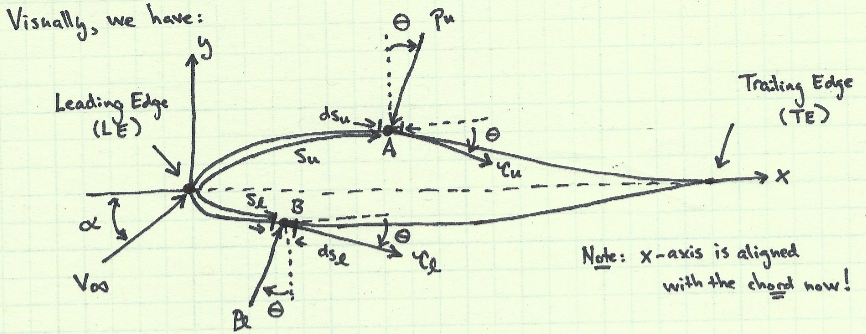
\includegraphics[width=0.5\linewidth]{Images/aero_forces.png}\par
\textbf{Lift and Drag per Unit Span}:\par
$L' = N'\cos{\alpha}-A'\sin{\alpha}$\par
$D' = N'\sin{\alpha}+A'\cos{\alpha}$\par
\textbf{Normal Force per Unit Span}: \par
$N' = \int_{LE}^{TE}(P_u\cos{\theta}+\tau_u\sin{\theta})ds_u+\int_{LE}^{TE}(P_l\cos{\theta}-\tau_l\sin{theta})ds_l$\par
\textbf{Axial Force per Unit Span}: \par
$A' = \int_{LE}^{TE}(-P_u\sin{\theta}+\tau_u\cos{\theta})ds_u+\int_{LE}^{TE}(P_l\sin{\theta}+\tau_l\cos{\theta})ds_l$\par
\textbf{Moment per Unit Span}:\par
$M_*'=\int_{LE}^{TE}\left[ (P_u\cos{\theta}+\tau_u\sin{\theta})(x-x^*)-(P_u\sin{\theta}-\tau_u\cos{\theta})(y-y*)\right]ds_u$ \par$+ \int_{LE}^{TE}\left[(-P_l\cos{\theta}+\tau_u\sin{\theta})(x-x^*)+(P_l\sin{\theta}+\tau_l\cos{\theta})(y-y*)\right]ds_l$\par
When $x^*=y^*=0$ we obtain the moment about the leading edge.\par
\textbf{Center of Pressure}:\par
$x_{cp} = -\frac{M_{LE}'}{N'}$\par

\subsection*{Force and Moment Coefficients}
\textbf{Dynamic Pressure}: $q = \frac{1}{2}\rho_\infty v_\infty^2$
\textbf{Reference Area}: $S$\par
\textbf{Reference Length}: $L$ or $c$\par
\textbf{Lift Coefficient}: $c_L=\frac{L}{q_\infty S}$\par
\textbf{Drag Coefficient}: $c_D = \frac{D}{q_\infty S}$\par
\textbf{Moment Coefficient}: $c_M=\frac{M}{q_\infty S L}$

\subsection*{Buckingham Pi Theorem}
If we have a physically meaningful equation such as:\par
$f(P_1,P_2,...,P_N) = 0$\par
where $P_i$ are physical variables in terms of $K$ independent physical units (mass, length, time, temperature) then it can be restated as:\par 
$F(\Pi_1,\Pi_2,...,\Pi_{N-K}) = 0$ or\par $\Pi_{N-K}=G(\Pi_1,\Pi_2,...,\Pi_{N-K-1})$\par 
where ${\Pi_i}$ are dimensionaless variables known as Pi Groups.

% ---------- Calculus ---------- %
\section*{Calculus Review}
\subsection*{Vector Calculus}
\textbf{Magnitude}: $|\vec{A}|=\sqrt{A_1^2+A_2^2+a_3^2}$\par 
\textbf{Dot Product}: $\vec{A}\cdot\vec{B}=A_xB_x+A_yB_y+A_zB_z=|\vec{A}||\vec{B}|\cos{\theta}$\par 
\textbf{Cross Product}:$\vec{A}\times\vec{B}=(A_yB_z-A_zB_y)\hat{i}+(A+zB_x-a_xB_z)\hat{j}+(A_xB_y-A_yB_x)\hat{k}$\par
$|\vec{A}\times\vec{B}|=|\vec{A}||\vec{B}|\sin{\theta}$\par 
\textbf{Gradient of Scalar Field}: $\vec{\nabla}p=\frac{\partial p}{\partial x}\hat{i}+\frac{\partial p}{\partial y}\hat{j}+\frac{\partial p}{\partial z}\hat{k}$ vector field\par 
Directional Derivative: $\frac{dp}{ds}=\vec{\nabla}p\cdot\vec{s}$-> unit vector in $\vec{s}$ direction.\par 
\textbf{Divergence of a Vector Field}: $\text{div}\vec{V}=\vec{\nabla}\cdot\vec{V}=\frac{\partial V_x}{\partial x}+\frac{\partial V_y}{\partial y}+\frac{\partial V_z}{\partial z}$ scalar field\par 
\textbf{Curl of a Vector Field}: $\text{curl}\vec{V}=\vec{\nabla}\times\vec{V}=(\frac{\partial V_z}{\partial y}-\frac{\partial V_y}{\partial z})\hat{i}
+(\frac{\partial V_x}{\partial z}-\frac{\partial V_z}{\partial x})\hat{j}
+(\frac{\partial V_y}{\partial x}-\frac{\partial V_x}{\partial y})\hat{k}$\par 
\subsection*{Integrals}
\textbf{Stokes' Theorem}: $\oint_c \vec{A}\cdot\vec{ds}=\iint_S(\vec{\nabla}\times\vec{A})\cdot\vec{dS}$\par 
\textbf{Divergence Theorem}: $\oiint_S\vec{A}\cdot\vec{dS}=\oiiint_\mathcal{V}(\vec{\nabla}\cdot\vec{A}d\mathcal{V})$\par 
\textbf{Gradient Theorem}: $\oiint_S p\vec{dS}=\oiiint_\mathcal{V} \vec{\nabla}pd\mathcal{V}$

% ----- Basic Flow Equations ----- %
\section*{Basic Flow Equations}
Fixed control volumes for basic flow equations.\par 
\subsection*{Conservation of Mass}
Net mass flow out of $\mathcal{V}$ = Time rate of decrease of mass inside $\mathcal{V}$.\par 
\textbf{Integral Continuity Equation}:\par 
$\frac{\partial}{\partial t}\oiiint_\mathcal{V}\rho d\mathcal{V}+\oiint_S\rho\vec{V}\cdot\vec{dS}=0$\par
\textbf{Differential Continuity Equation}:\par
$\frac{\partial\rho}{\partial t}+\vec{\nabla}\cdot(\rho\vec{V})=0$

\subsection*{Conservation of Momentum}
Net force applied to $\mathcal{V}$ = Time rate of change of momentum of fluid in $\mathcal{V}$\par 
$\frac{\partial}{\partial t}\oiiint_\mathcal{V}\rho\vec{V}d\mathcal{V}+\oiint_S(\rho\vec{V}\cdot\vec{dS})\vec{V}=-\oiint_S p\vec{dS}+\oiiint_\mathcal{V}\rho\vec{f}d\mathcal{V}+\vec{F}_{viscous}$
\begin{enumerate}
    \item Body Forces (e.g. gravity) which act on the fluid inside $\mathcal{V}$\par
    $\oiiint_\mathcal{V}\rho\vec{f}d\mathcal{V}$
    \item Pressure and shear surface forces acting on S\par 
    $-\oiint_S p\vec{dS}+\vec{F}_{viscous}$
    \item Net flow of momentume out of volume across S\par 
    $\oiint_S(\rho\vec{V}\cdot\vec{dS})\vec{V}$
    \item Time rate of change of momentum due to unsteadiness in volume\par 
    $\frac{\partial}{\partial t}\oiiint_\mathcal{V}\rho\vec{V}d\mathcal{V}$
\end{enumerate}
\textbf{Navier-Stokes Equations}:\par
$\frac{\partial}{\partial t}(\rho u)+\vec{\nabla}\cdot(\rho u \vec{V}) = -\frac{\partial p}{\partial x}+\rho f_x+(\mathcal{F}_x)_{viscous}$\par
$\frac{\partial}{\partial t}(\rho v)+\vec{\nabla}\cdot(\rho v \vec{V}) = -\frac{\partial p}{\partial y}+\rho f_y+(\mathcal{F}_y)_{viscous}$\par

\subsection*{Conservation of Energy}
\includegraphics[width=.75\linewidth]{Images/consv_energy.png}\par
\includegraphics[width=.75\linewidth]{Images/consv_energy_diff.png}

% ----- Kinematics ----- %
\section*{Kinematics}
$\vec{\nabla}\cdot\vec{V}$: time rate of change of volume of a fluid element per unit volume $\rightarrow$ \textbf{Dilation}\par
\textbf{Stream Line}: Curve everywhere tangent to the velocity.\par
$\frac{v}{u}=\frac{dy}{dx}$\par 
\textbf{Path Line}: Trajectory of a particle released from a point in time.\par 
\textbf{Streak Line}: Line connecting all particles that have passed through a given point.\par 
For a steady flow the three lines coincide.\par
\subsection*{Substantial Derivative}
Time rate of change of density of a given material fluid element as it moves through space and time.\par 
$\frac{D\rho}{Dt}=\frac{\partial\rho}{\partial t}+\vec{V}\cdot\vec{\nabla}\rho$\par 
Continuity Equation:$\frac{D\rho}{Dt}=-\rho\vec{\nabla}\cdot\vec{V}$\par 
Material Acceleration: $(\frac{Du}{Dt};\frac{Dv}{Dt};\frac{Dz}{Dt})$\par 
Navier-Stokes:\par 
$\rho\frac{Du}{Dt}=-\frac{\partial p}{\partial x}+\rho f_x+(\mathcal{F}_x)_{viscous}\rightarrow$ applicable to y and z as well.\par 

\subsection*{Vorticity and Strain}
$\vec{\omega}=\frac{1}{2}\vec{\nabla}\times\vec{V}\rightarrow$ angular velocity\par 
$\vec{\xi}=\vec{\nabla}\times\vec{V}\rightarrow$ Vorticity\par 
$\varepsilon_{xy}=\frac{\partial v}{\partial x}+\frac{\partial u}{\partial y}\rightarrow$ Rate of Strain in xy plane.\par
$\Gamma=-\oint_C\vec{V}\cdot\vec{ds}\rightarrow$ Circulation\par 
Relation between circulation and vorticity: $\vec{xi}\cdot\vec{n}=\frac{d\Gamma}{dS}$

\subsection*{Stream Functions and Velocity Potentials}
\textbf{Stream Function}: For every incompressible, two-dimensional flow, there exists a scalar stream function such that: $u=\frac{\partial\psi}{\partial y}$, $v=-\frac{\partial\psi}{\partial x}$ DON'T FORGET +C\par 
\textbf{Velocity Potential}: For every irrotational flow, there exists a scalar velocity potential such that: $\vec{V}=\vec{\nabla}\phi/rightarrow \frac{\partial\phi}{\partial x}=y$, $\frac{\partial\phi}{\partial y}=x$\par 
\textbf{Euler's Equation}: $\frac{1}{2}d(V^2)=-\frac{1}{\rho}dp$\par 
If flow is barotropic, $\rho=\rho(p)$ is a function of pressue only and can integrate the equation. Occurs in incompressible flow, isothermal flow, or isentropic (frictionless) flow.\par 
\textbf{Bernoulli's Equation}: $p+\frac{1}{2}\rho V^2=\text{constant}$ - along a streamline for steady, inviscid, incompressible flow with no body forces.

\subsection*{Flow in a Duct}
$\rho_1A_1V_1=\rho_2A_2V_2\rightarrow$ Steady, inviscid flow in a duct with no body forces. For incompressible flow remove rho.



\end{multicols*}
\end{document}
